\documentclass{standalone}
\usepackage{tikz}
\usetikzlibrary{positioning}

\begin{document}

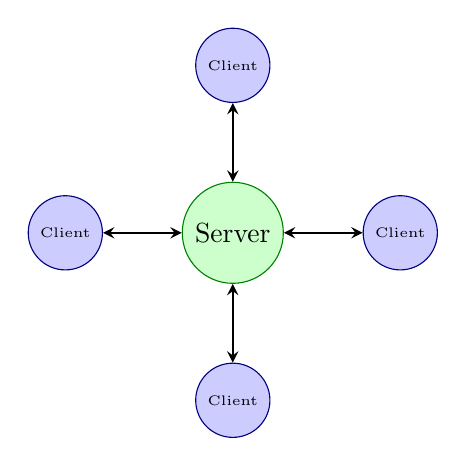
\begin{tikzpicture}
[repo/.style={circle,
		fill=green!20!white,
		draw=green!50!black,
		minimum size=10mm},
workingcopy/.style={circle,
		fill=blue!20!white,
		draw=blue!50!black,
		minimum size=5mm},
link/.style={-, >=stealth, thick}]

% central repo
\node (main repo) at (0, 0) [repo] {Server};
% working copies
\node (client right)  [workingcopy, right=of main repo] {\tiny Client};
\node (client left)   [workingcopy, left=of main repo]  {\tiny Client};
\node (client top)    [workingcopy, above=of main repo] {\tiny Client};
\node (client bottom) [workingcopy, below=of main repo] {\tiny Client};
% links between repo and working copies
\draw [link, <->] (main repo) -- (client right);
\draw [link, <->] (main repo) -- (client left);
\draw [link, <->] (main repo) -- (client top);
\draw [link, <->] (main repo) -- (client bottom);
\end{tikzpicture}
\end{document}
